\section{Application Context}

The app is to be developed to provide a proof-of-concept for the framework.
Basic tasks of the app include showing off the capabilities of the framework, proving the implementation, and as an example on how to utilize the framework.
The app will be developed for Android 4 and above, although the framework will be independent from any Android version within the scope of its dependencies on external libraries.
The app will force landscape view as it offers the more natural layout for the layout of the app.
Apart of the OpenCV for Android library for Imagine, the application shall have no further dependencies on other 3rd party tools.
This should ensure a clean and fast code for the application.

\section{System Tasks}

In this section, we will take a look at the various tasks the final app should be capable of doing.
Note that we differentiate between required tasks (meaning tasks that should reliably and completely work for the app to be considered done) and optional tasks (tasks that might be included, depending on time and scope of their implementation).

\subsection{Required Tasks}

Table \ref{app_tasks} lists the tasks that the sample application should minimally allow to be accessed and used.
Further tasks may be implemented as required.

\begin{table}
	\centering
	\begin{tabulary}{\textwidth}{L || L}
	View Camera & The user should, upon opening the app, be confronted with the view of the live camera feed.\\
	\hline
	Manage Model & Load, prepare, and remove a 3d model to be used within the app with a marker. Any model in a recognized format should be selectable as a file from a file browser. \\
	\hline
	Manage Markers & Allow for the management of multiple markers and their associations to the models. \\
	\hline
	Toggle Debugging Information & If desirable, the user can toggle a debugging view to be rendered on top of the feed. This should offer detailed information on the shown view, marker detection, and any other factors. \\
	\hline
	Screenshot & As Android does not offer a screenshot tool by default, an option to capture the feed shall be provided. \\
	\end{tabulary}
	\caption[Application Tasks]{Tasks that the sample application should enable.}
	\label{app_tasks}
\end{table}

\section{Dialog Structure}

\begin{figure}
	\centering
	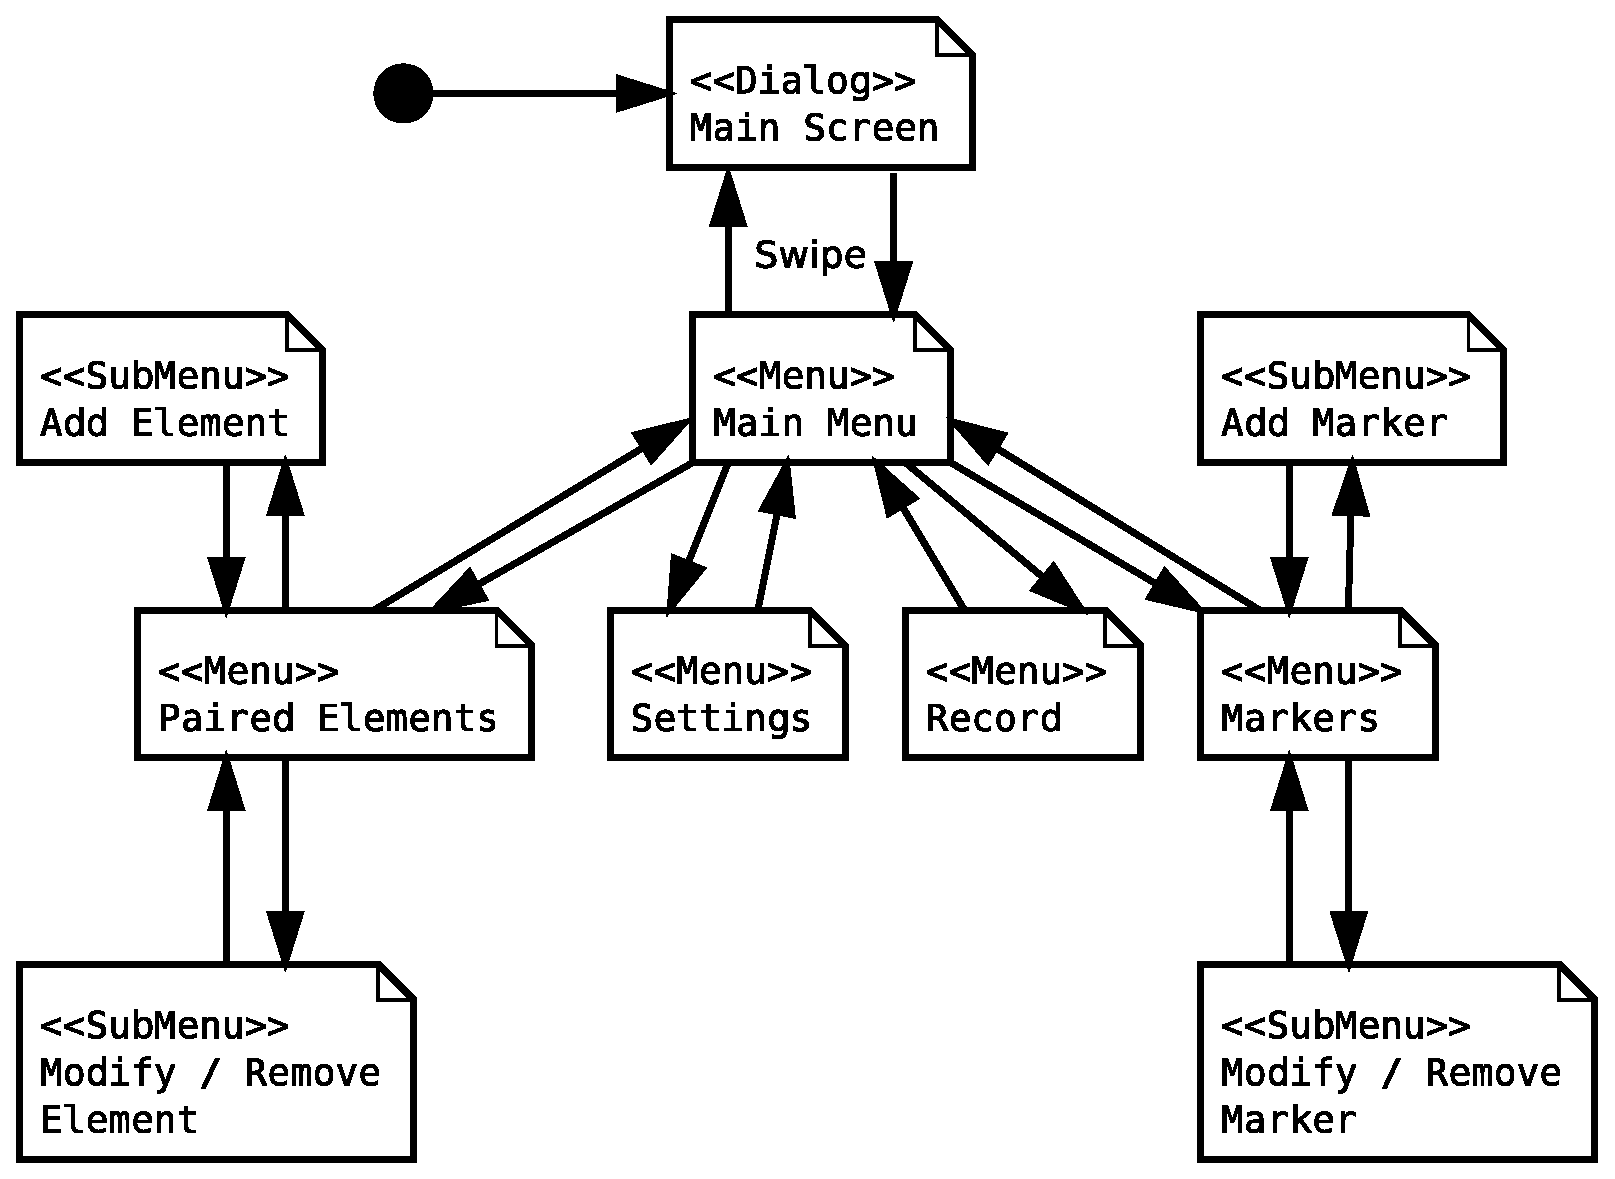
\includegraphics[width=10cm]{img/dialogs.eps}
	\caption[App Dialog Structure.]{Overview of the dialog structure of the app. Except where otherwise noted, all actions from one dialog to another are a simple touch.}
	\label{fig:dialog_structure}
\end{figure}

Figure \ref{fig:dialog_structure} shows a graph of the usage flow in the app graphical user interface.
Note that apart from the layout change from just the main screen to the screen with the menu displayed at the right border, all sub-menus are displayed in-place to the original menu.
This allows the main purpose of the app, namely the rendering of AR, to always be in the focus of the user.
This enables rapid and direct feedback to any changes the user does within the menus.

\section{Mockups}

\begin{figure}
	\centering
	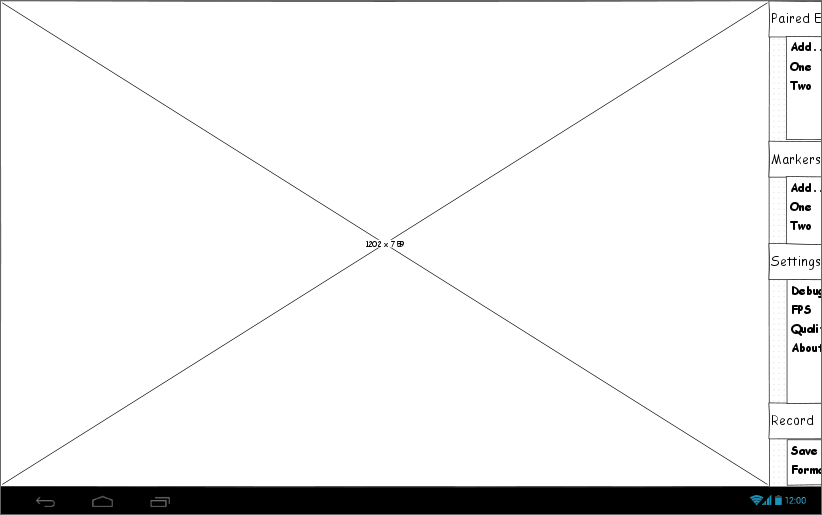
\includegraphics[width=12cm]{img/main_nomenu.png}
	\caption[Start Screen Mockup.]{Mockup of how the start screen of the final app might look. Note the menu partially hidden to the right, the rendered axes, and the green status light signifying that the marker is being read with a high confidence.}
	\label{fig:main_nomenu}
\end{figure}

Upon starting the app on a capable device, the app presents itself as shown in Figure \ref{fig:main_nomenu}.
This is effectively the start screen from where all the interaction takes place.

The green light in the top left shows that the app is detecting the marker with a high confidence, meaning that there are no large uncertainties.
If the marker is too warped or partially covered, the light switches to red.
If the app can still detect the marker but is having difficulties, the light switches to orange.
This mechanism is meant to offer fast and accurate feedback to the detection capability.
Another method of direct feedback is the already displayed axis-object.
This is meant to offer fast feedback to the orientation and scaling of the coordinate space to the user before a custom object is displayed.
The visibility of the axis-object can be toggled in the settings.

The menu on the right can be swiped in to be fully displayed.
The four main points are <Paired Elements>, <Markers>, <Settings>, and <Record>.

\begin{figure}[H]
	\centering
	\minipage{0.49\textwidth}
		\centering
		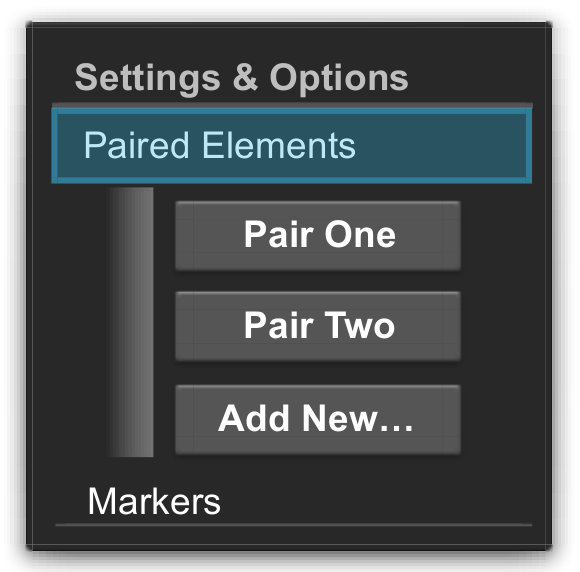
\includegraphics[width=0.5\linewidth]{img/menu_paired.png}
		\caption[Paired Element Menu Mockup.]{Mockup of the <Paired Elements> part of the main menu. From here, the user can select to work on an existing pair or add a new one.}
		\label{fig:menu_paired}
	\endminipage\hfill
	\minipage{0.49\textwidth}
		\centering
		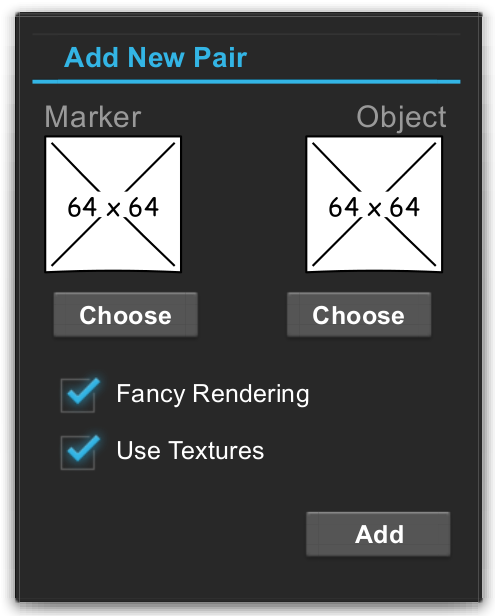
\includegraphics[width=0.5\linewidth]{img/menu_paired_add.png}
		\caption[Paired Element Pair Add Menu Mockup.]{Mockup of the menu to add a new pair to use. Here the initial marker and object can be chosen, along with any exposed options before creating the pairing for active use.}
		\label{fig:menu_paired_add}
	\endminipage\hfill
	\minipage{0.9\textwidth}
		\centering
		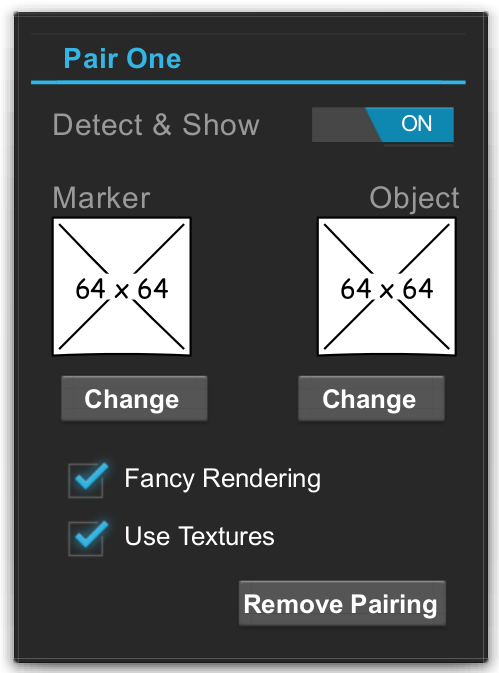
\includegraphics[width=0.25\linewidth]{img/menu_paired_pair.png}
		\caption[Paired Element Pair Menu Mockup.]{Mockup of the menu for modifying existing pairs, including removing them. Note the switch to use a pair and the preview of the marker and object with the ability to change both.}
		\label{fig:menu_paired_pair}
	\endminipage\hfill
\end{figure}

Figure \ref{fig:menu_paired} shows the <Paired Elements> menu, which lists the current paired marker-object pairs that the app can detect.
From here, the user can modify existing pairs by touching them, which opens a new menu shown in Figure \ref{fig:menu_paired_pair} in place with options pertaining to that pair, including its removal.
Adding new pairs is done via the <Add> button at the top, displaying the menu as in Figure \ref{fig:menu_paired_add} to select the marker and object to pair.

\begin{figure}[H]
	\centering
	\minipage{0.49\textwidth}
		\centering
		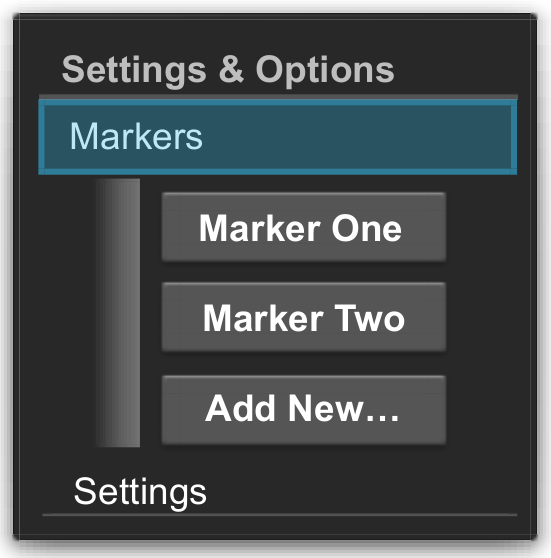
\includegraphics[width=0.5\linewidth]{img/menu_marker.png}
		\caption[Marker Element Menu Mockup.]{Mockup of the <Marker> sub-menu of the main menu. From here, modifying and adding new markers is provided.}
		\label{fig:menu_marker}
	\endminipage\hfill
	\minipage{0.49\textwidth}
		\centering
		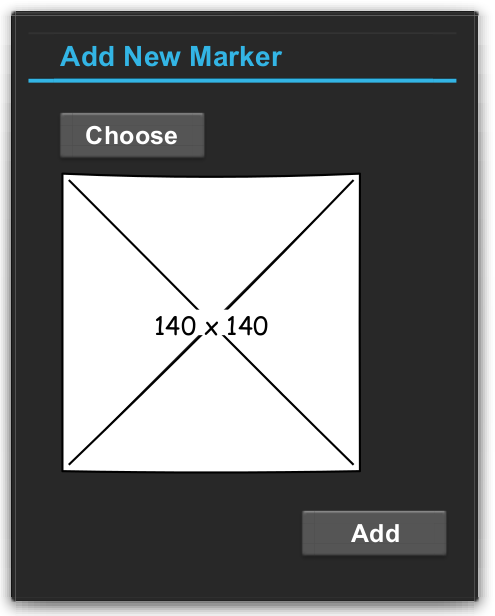
\includegraphics[width=0.5\linewidth]{img/menu_marker_add.png}
		\caption[Marker Add Menu Mockup.]{Mockup for adding a new marker by choosing a suitable image file to use.}
		\label{fig:menu_marker_add}
	\endminipage\hfill
	\minipage{0.9\textwidth}
		\centering
		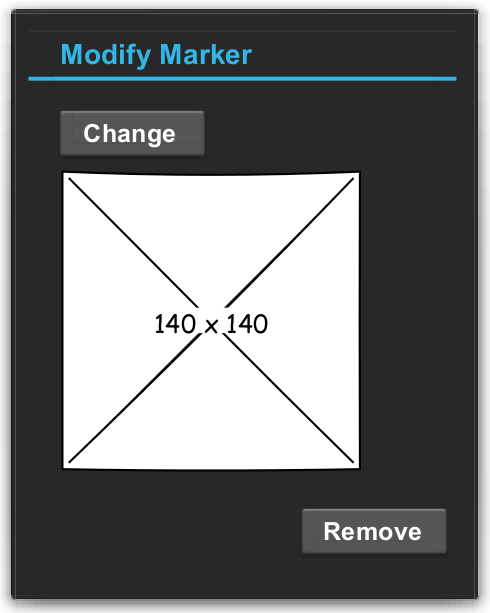
\includegraphics[width=0.25\linewidth]{img/menu_marker_modify.png}
		\caption[Modify Marker Menu Mockup.]{Modifying existing markers is done in this mockup. This includes the option to delete a marker.}
		\label{fig:menu_marker_modify}
	\endminipage\hfill
\end{figure}

<Markers>, as seen in Figure \ref{fig:menu_marker}, lists the available markers and provides options for organizing them.
Again, touching a marker opens an in-place menu with options, as in Figure \ref{fig:menu_marker_modify}.
Adding new markers via Figure \ref{fig:menu_marker_add}, either by loading a picture, using a default, or taking a picture from the camera, can be done via the <Add> button.

\begin{figure}[H]
	\centering
	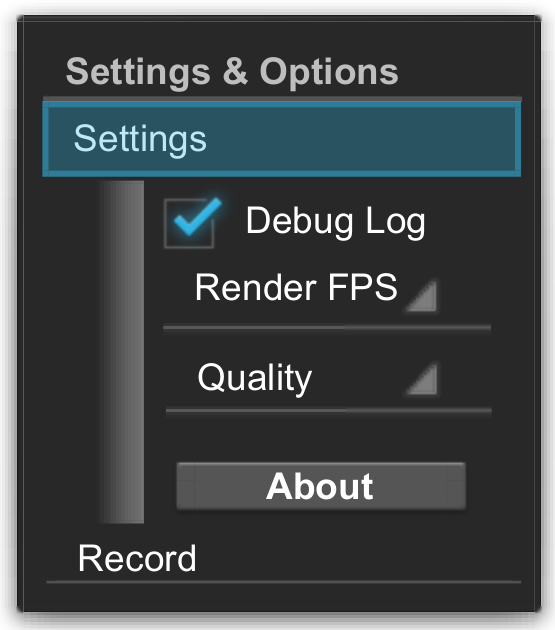
\includegraphics[width=4cm]{img/menu_settings.png}
	\caption[Settings Menu Mockup.]{This mockups depicts the <Settings> menu. From here, the user should be allowed to change a few general settings of the app and to read the <About> page.}
	\label{fig:menu_settings}
\end{figure}

The <Settings> menu seen in Figure \ref{fig:menu_settings} is just that.
Here, the user can change app-specific settings such as video resolution, directories, debugging information, and more.

\begin{figure}[H]
	\centering
	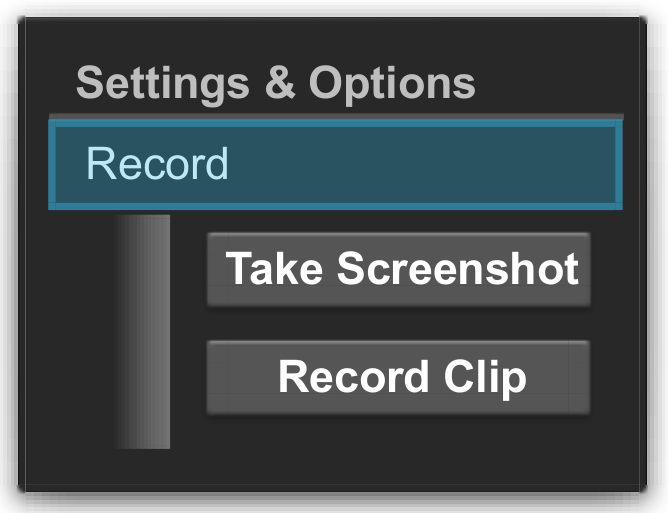
\includegraphics[width=4cm]{img/menu_record.png}
	\caption[Record Menu Mockup.]{This mockup shows the panel for the <Record> menu, from which a screenshot or a short video clip can be taken of the output of the app.}
	\label{fig:menu_record}
\end{figure}

<Record> allows the user to record the current rendering, either as a picture or possibly as a video.
The options beneath this item are for controlling those features.
